\فصل{ارزیابی}

\label{section:experiment}
\قسمت{مقدمه}

در این بخش، به ارزیابی مدل ارائه شده با مدل های معروف و جدید می‌پردازیم، در ابتدا در رابطه با مجموعه‌داده ای که آموزش و آزمون بر روی آن انجام شده است اطلاعاتی را می‌دهیم و جزئییات آن را مورد بررسی قرار می‌دهیم. سپس معیارهای ارزیابی را معرفی می‌کنیم که توسط آنها، عملکرد مدل معرفی شده را می‌سنجیم و بعد در قالب جدول‌ها عملکرد مدل را با مدل‌های پیشین مقایسه می‌کنیم.

\قسمت{مجموعه‌داده}

مجموعه داده PascalVOC که توسط Everingham و همکاران در سال 2010 معرفی شده است، یکی از مجموعه داده‌های مشهور و پرکاربرد در حوزه یادگیری ماشین و بینایی کامپیوتر است\cite{Everingham2010ThePV}. این مجموعه داده شامل 1464 تصویر برای آموزش (Train)، 1449 تصویر برای اعتبارسنجی (Validation) و 1456 تصویر برای آزمون (Test) است. این تصاویر به‌صورت دستی برچسب‌گذاری شده‌اند و شامل 21 کلاس مختلف از اشیاء می‌باشند.

هدف اصلی مجموعه داده PascalVOC ارزیابی عملکرد مدل‌های تشخیص اشیاء و بخش‌بندی تصویر است. این کلاس‌ها شامل مواردی مانند انسان، حیوانات (سگ، گربه، پرنده)، وسایل نقلیه (دوچرخه، ماشین، هواپیما) و اشیاء روزمره (صندلی، میز، بطری) هستند. یکی از ویژگی‌های مهم این مجموعه داده، تنوع بالای تصاویر از نظر زاویه دید، اندازه اشیاء، و شرایط نوری مختلف است که آن را به چالشی مناسب برای ارزیابی الگوریتم‌های پیشرفته تبدیل کرده است.

مجموعه‌داده مذکور یکی از مهمترین مجموعه‌ها در زمینه بخش‌بندی معنایی می‌باشد که بسیاری از مدل های روز دنیا از این مجموعه‌داده برای ارزیابی مدل خود استفاده می‌کنند.


\قسمت{‌معیارهای ارزیابی}

عملکرد بخش‌بندی تصویر بر اساس استانداردهای تعیین‌شده با استفاده از معیارهای IoU (تقاطع بر اتحاد) ارزیابی می‌شود. برای مقایسه‌ای منصفانه، میانگین این معیارها بر پایه سه اجرای مختلف محاسبه می‌گردد. همچنین، اندازه مدل با توجه به تعداد پارامترهای گزارش‌شده در ساختار شبکه مشخص می‌شود. معیار IoU، که مخفف Intersection over Union است، نسبت مساحت اشتراک ناحیه پیش‌بینی‌شده و ناحیه واقعی به مساحت اجتماع آن‌ها را نشان می‌دهد و یکی از مهم‌ترین معیارهای ارزیابی عملکرد در وظایف بخش‌بندی تصویر است.

\قسمت{‌جزئیات پیاده‌سازی}

برای مجموعه داده‌ی Pascal، از سایز دسته‌ای (batch size) برابر با ۶ و مجموع ۱۲۰ دوره (epoch) استفاده می‌شود. بهینه‌ساز Stochastic Gradient Descent (SGD) با نرخ یادگیری اولیه ۰.۰۰۷ به کار گرفته می‌شود. تنظیم نرخ یادگیری بر اساس برنامه‌ریز کسینوسی (cosine annealing scheduler) انجام می‌شود. پیش از مرحله‌ی آموزش، هر تصویر پردازش اولیه شامل تغییر مقیاس تصادفی در بازه‌ی ۰.۵ تا ۲ برابر اندازه‌ی اصلی، معکوس کردن افقی تصادفی و برش تصادفی به ابعاد ۵۱۳×۵۱۳ پیکسل را تجربه می‌کند.

وزن‌های اولیه‌ی بخش‌های پشتیبان (backbone) شبکه‌های معلم و دانش‌آموز از مجموعه داده‌ی ImageNet بارگذاری می‌شوند، در حالی که بخش‌های مربوط به بخش‌بندی (segmentation) به صورت تصادفی مقداردهی اولیه می‌شوند.


\قسمت{‌نتایج تجربی}

در تصویر 4-1، نتیجه اجرای مدل را بر روی سه تصویر از مجموعه‌داده Voc Pascal قابل مشاهده است که با مقایسه آن با قطعه های حقیقی، عملکرد مناسب مدل ما مشهود است.

\input{figures/result}

\subsection{مقایسه با کار‌های پیشین}

آزمایش‌های گسترده‌ای برای ارزیابی عملکرد روش پیشنهادی انجام شد. این روش با چندین روش تقطیر موجود مقایسه گردید، از جمله: KD \cite{hinton2015distillingknowledgeneuralnetwork}، CIRKD \cite{yang2022crossimagerelationalknowledgedistillation}، DistKD \cite{huang2022knowledgedistillationstrongerteacher} و LAD \cite{Liu2024RethinkingKD}. همچنین، در انجام آزمایش از مدل ResNet101 با 59.3 میلیون پارامتر به عنوان مدل معلم و از مدل های DeepLabV3-ResNet18، DeepLabV3-MBV2 و PSPNet-Res18 به عنوان مدل های دانش‌آموز استفاده شده است.
همانطور که در جدول 4-1 مشخص است، عملکرد ما نسبت به مدل‌های به‌روز در این زمینه در هر سه مدل بهتر است.
‫‫


\begin{table*}[!htbp]
	\caption[نتایج بخش‌بندی معنایی]{نتایج بخش‌بندی معنایی. روش ما و روش های بخش‌بندی معنایی بر روی مجموعه‌داده Pascal Voc که نشان‌دهنده ی عملکرد بهتر مدل ما نسبت به مدل های موجود است. }
	\begin{center}
    \label{tab:results}
		\begin{tabular}{l c c}
\hline
Method & mIoU(\%) & Params(M) \\
\hline
T: DeepLabV3-Res101 & $77.85$ & $59.3$ \\
\hline
S: DeepLabV3-Res18 & $67.50$ & \\
KD + S & $0.11$ \(\pm\)  $69.13$ & \\
DistKD + S & $0.11$ \(\pm\) $69.84$ & $16.6$ \\
CIRKD + S & $0.11$ \(\pm\) $71.02$ & \\
LAD + S & $0.09$ \(\pm\) $71.42$ & \\
Ours + S & \textbf{$0.08$} \(\pm\) \textbf{$72.19$} & \\
\hline
S: DeepLabV3-MBV2 & $63.92$ & \\
KD + S & $0.21$ \(\pm\) $66.39$ & \\
DistKD + S & $0.22$ \(\pm\) $67.62$ & $5.9$ \\
CIRKD + S & $0.16$ \(\pm\) $69.02$ & \\
LAD + S & $0.07$ \(\pm\) $68.63$ & \\
Ours + S & \textbf{$0.11$} \(\pm\) \textbf{$69.32$} & \\
\hline
S: PSPNet-Res18 & $67.4$ & \\
KD + S & $0.08$ \(\pm\) $68.18$ & \\
DistKD + S & $0.19$ \(\pm\) $68.93$ & $12.6$ \\
CIRKD + S & $0.11$ \(\pm\) $69.53$ & \\
LAD + S & $0.10$ \(\pm\) $69.71$ & \\
Ours + S & \textbf{$0.08$} \(\pm\) \textbf{$71.35$} & \\
\hline
\end{tabular}
		\label{4_tracking_results}
	\end{center}
\end{table*}

\قسمت{رابط کاربری سامانه پورتفولیو}
برای نمایش قابلیت‌های سامانه، در ادامه نماهای مختلف رابط کاربری آورده شده است. کلیهٔ تصاویر با استفاده از مرورگر وب و بر روی نمونهٔ استقراریافتهٔ Docker تهیه شده‌اند.

\begin{figure}[H]
\centering

\includegraphics[width=0.9\textwidth]{../figures/1.صفحه اصلی.png}
\caption{صفحهٔ اصلی سامانه پس از ورود به آدرس \lr{http://localhost}}
\end{figure}

\begin{figure}[H]
\centering
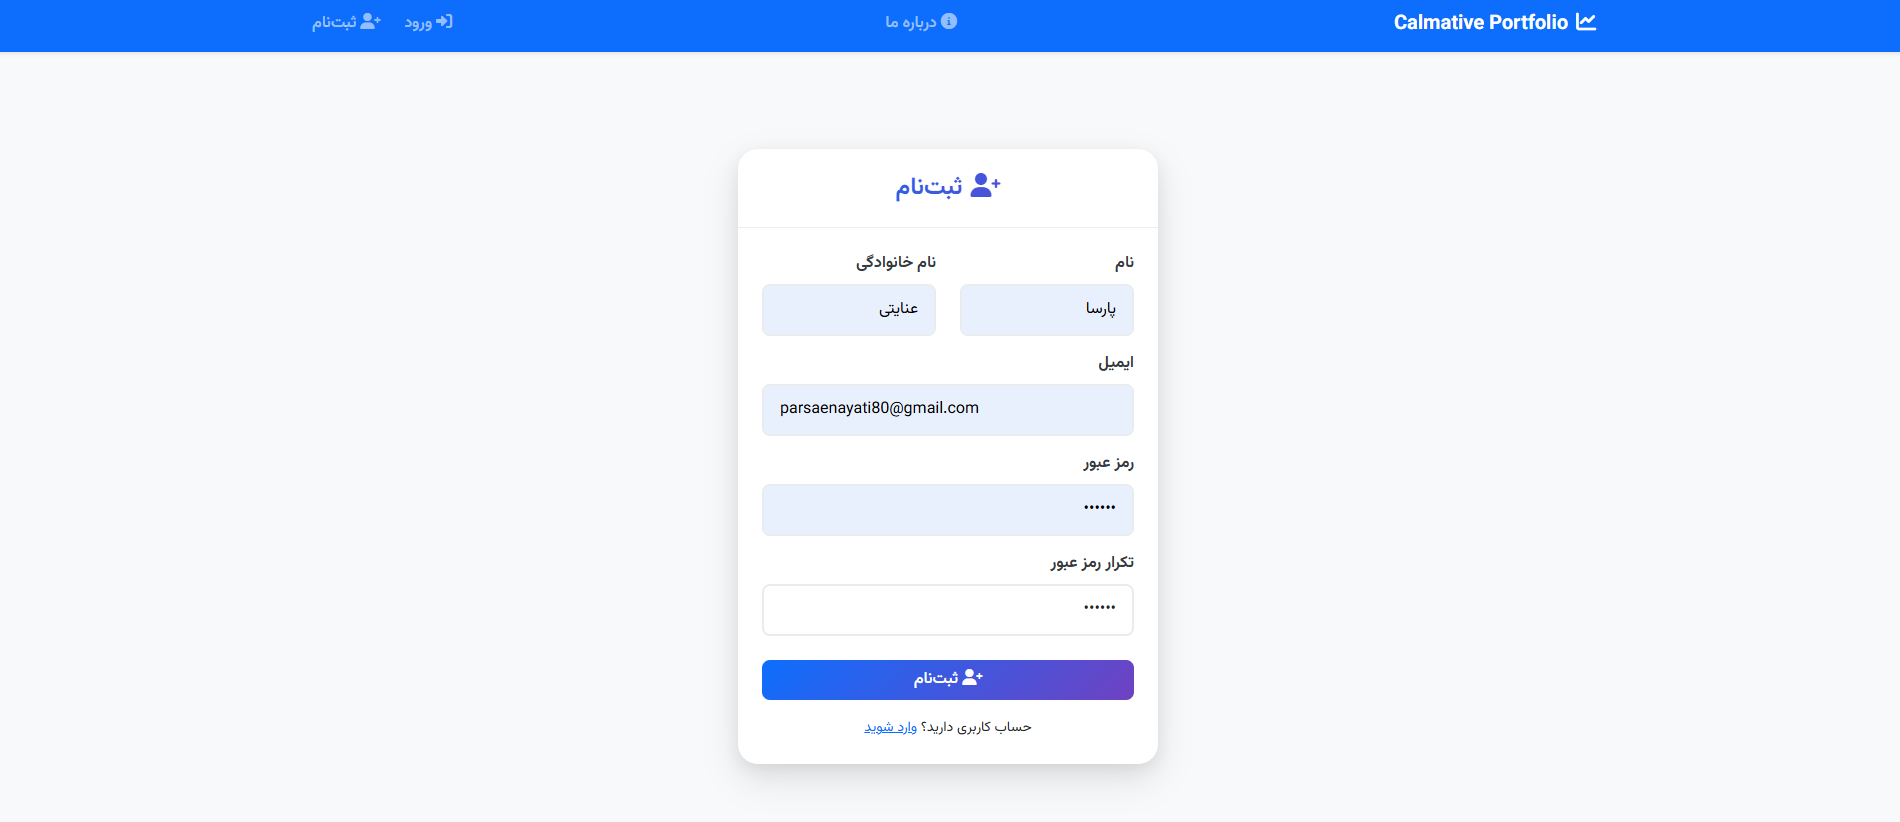
\includegraphics[width=0.9\textwidth]{../figures/2. صفحه ثبت نام.png}
\caption{فرم ثبت‌نام کاربر جدید}
\end{figure}

\begin{figure}[H]
\centering
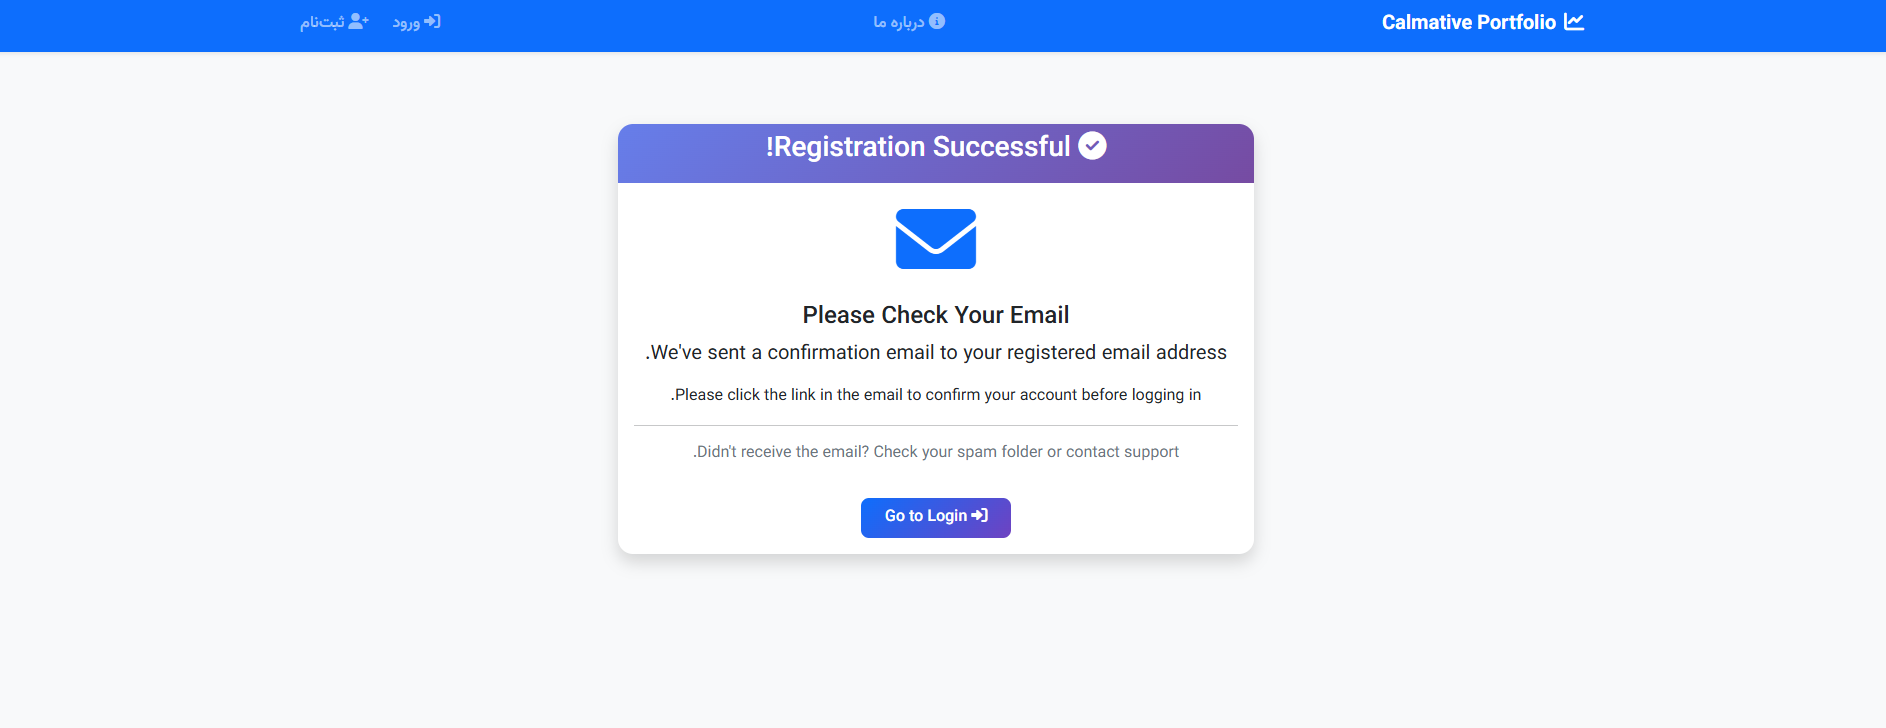
\includegraphics[width=0.9\textwidth]{../figures/3. صفحه ارسال ایمیل تایید.png}
\caption{اعلان ارسال لینک تأیید ایمیل}
\end{figure}

% ... سایر تصاویر به همین ترتیب ...

\begin{figure}[H]
\centering
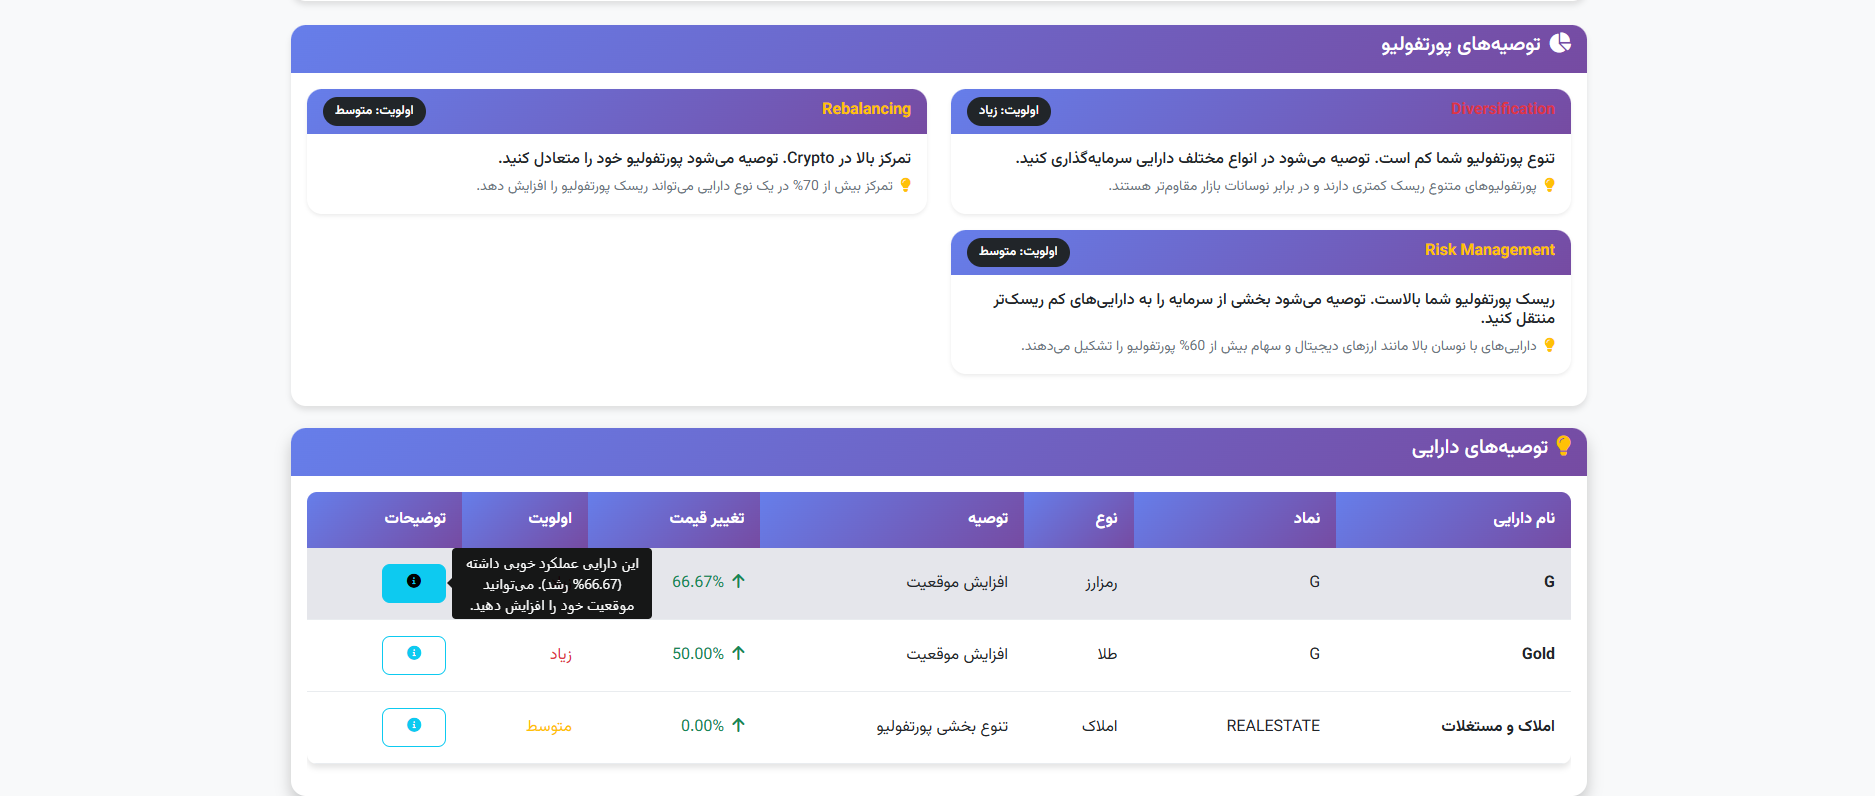
\includegraphics[width=0.9\textwidth]{../figures/21. دریافت توصیه هوشمند برای پورتفولیو.png}
\caption{نمایش توصیه‌های هوشمند برای یک پورتفولیو}
\end{figure}

\pagebreak